%!TEX root = ../../presentation.tex

\section{Theoretical Background}

\begin{frame}
    \frametitle{Why Twitter?}

    \begin{outline}
        \1 Reliable in previous studies \citep{Barbosa2010}
            \2 Public opinion \citep{Oconnor2010a,Patodkar2016a}
            \2 Stock market prediction \citep{Bollen2011a,Mittal2012a,Nguyen2015a,Pagolu2016a,Zhang2011a}

        \1 Short messages of up to 280 characters \citep{Rosen2017}
        \1 One topic is assumed due limited characters \citep{Pagolu2016a,Patodkar2016a}
    \end{outline}
\end{frame}
  
\note[itemize]{
    \item Page 11
}

\begin{frame}
    \frametitle{Sentiment Detection Algorithms}

    \begin{outline}
        \1 \tb{}
        \1 \nb{}
        \1 \me{}
        \1 \svm{}
    \end{outline}
\end{frame}

\note[itemize] {
    \item {
        Naive Bayes:
        \begin{equation}
            P_{NB}(c|d) = \frac{P(c) (\prod_{i=1}^{m} P(f_i|c)^{n_i(d)}) }{P(d)}
            \label{eq:background-optionmining-machinelearningalgorithms-bayes}
        \end{equation}
    }
}

\note[itemize] {
    \item {
     Maximum Entropy:
        \begin{equation}
            P_{ME}(c|d) = \frac{1}{Z(d)} exp \left( \sum_i^m \lambda_{i,c}F_{i,c}(d,c) \right)
            \label{eq:background-optionmining-machinelearningalgorithms-maximumentropy}
        \end{equation}

        \begin{equation}
            Z(d) = \sum_c exp(\sum_i \lambda_{i,c} F_{i,c}(d,c))
            \label{eq:background-optionmining-machinelearningalgorithms-maximumentropy_Zd}
        \end{equation}
    
        \begin{equation}
        F_{i,c}(d,c') = 
            \begin{cases}
            1, & n_i(d) > 0 \text{ and } c' = c \\
            0  & \text{otherwise}
            \end{cases}
            \label{eq:background-optionmining-machinelearningalgorithms-maximumentropy_fic}
        \end{equation}
    }
}

\note[itemize] {
    \item {
        Support Vector Machine:
        \begin{figure}[ht]
            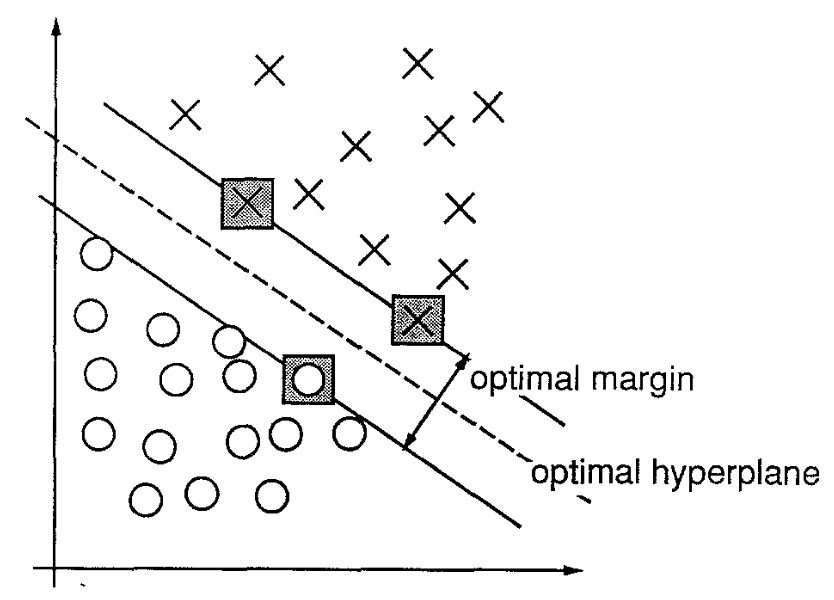
\includegraphics[width=.7\textwidth]{images/svm.png}
            \label{fig:background-optionmining-machinelearningalgorithms-svm}
        \end{figure}        
    }
}